
\documentclass[a4paper,11pt]{article}%,twocolumn
%% packages

\usepackage{blindtext} % needed for creating dummy text passages
%\usepackage{ngerman} % needed for German default language
\usepackage{amsmath} % needed for command eqref
\usepackage{amssymb} % needed for math fonts
\usepackage[colorlinks=true,breaklinks]{hyperref} % needed for creating hyperlinks in the document, the option colorlinks=true gets rid of the awful boxes, breaklinks breaks lonkg links (list of figures), and ngerman sets everything for german as default hyperlinks language
\usepackage[hyphenbreaks]{breakurl} % ben�tigt f�r das Brechen von URLs in Literaturreferenzen, hyphenbreaks auch bei links, die �ber eine Seite gehen (mit hyphenation).
\usepackage{xcolor}
\definecolor{c1}{rgb}{0,0,1} % blue
\definecolor{c2}{rgb}{0,0.3,0.9} % light blue
\definecolor{c3}{rgb}{0.3,0,0.9} % red blue
\hypersetup{
    linkcolor={c1}, % internal links
    citecolor={c2}, % citations
    urlcolor={c3} % external links/urls
}
%\usepackage{cite} % needed for cite
\usepackage[square,authoryear]{natbib} % needed for cite and abbrvnat bibliography style
\usepackage[nottoc]{tocbibind} % needed for displaying bibliography and other in the table of contents
\usepackage{graphicx} % needed for \includegraphics 
\usepackage{longtable} % needed for long tables over pages
\usepackage{bigstrut} % needed for the command \bigstrut
\usepackage{enumerate} % needed for some options in enumerate
%\usepackage{todonotes} % needed for todos
\usepackage{makeidx} % needed for creating an index
\makeindex
\usepackage{gensymb}
\usepackage{url}
\usepackage{psfrag}
\usepackage{multirow}
\usepackage{subfigure}
%% page settings

\usepackage[top=20mm, bottom=20mm,left=15mm,right=15mm]{geometry} % needed for page border settings
\parindent=0mm % for space of first line of new text block
\sloppy % for writing with hyphenless justification (tries to)
\hyphenation{} % use hyphenation of tolerance parametershttp://www.jr-x.de/publikationen/latex/tipps/zeilenumbruch.html
\hyphenpenalty=10000
\exhyphenpenalty=10000
\usepackage{fancyhdr} % needed for head and foot options
%% my macros

%% Text fomats
\newcommand{\tbi}[1]{\textbf{\textit{#1}}}

%% Math fonts
\newcommand{\bbA}{\mathbb{A}}
\newcommand{\bbB}{\mathbb{B}}
\newcommand{\bbC}{\mathbb{C}}
\newcommand{\bbD}{\mathbb{D}}
\newcommand{\bbE}{\mathbb{E}}
\newcommand{\bbF}{\mathbb{F}}
\newcommand{\bbG}{\mathbb{G}}
\newcommand{\bbH}{\mathbb{H}}
\newcommand{\bbI}{\mathbb{I}}
\newcommand{\bbJ}{\mathbb{J}}
\newcommand{\bbK}{\mathbb{K}}
\newcommand{\bbL}{\mathbb{L}}
\newcommand{\bbM}{\mathbb{M}}
\newcommand{\bbN}{\mathbb{N}}
\newcommand{\bbO}{\mathbb{O}}
\newcommand{\bbP}{\mathbb{P}}
\newcommand{\bbQ}{\mathbb{Q}}
\newcommand{\bbR}{\mathbb{R}}
\newcommand{\bbS}{\mathbb{S}}
\newcommand{\bbT}{\mathbb{T}}
\newcommand{\bbU}{\mathbb{U}}
\newcommand{\bbV}{\mathbb{V}}
\newcommand{\bbW}{\mathbb{W}}
\newcommand{\bbX}{\mathbb{X}}
\newcommand{\bbY}{\mathbb{Y}}
\newcommand{\bbZ}{\mathbb{Z}}
\usepackage[ framed, numbered]{matlab-prettifier}%framed,%
\usepackage{listings}
\usepackage{physics}
\usepackage{pdfpages}
\usepackage[toc,page]{appendix}
\usepackage{float}
% for code
\usepackage{listings}
\usepackage{color}
% Define colors
\definecolor{codegreen}{rgb}{0,0.6,0}
\definecolor{codegray}{rgb}{0.5,0.5,0.5}
\definecolor{codepurple}{rgb}{0.58,0,0.82}
\definecolor{backcolour}{rgb}{0.95,0.95,0.92}
% Setup the listings package
\lstset{
    backgroundcolor=\color{backcolour},   
    commentstyle=\color{codegreen},
    keywordstyle=\color{magenta},
    numberstyle=\tiny\color{codegray},
    stringstyle=\color{codepurple},
    basicstyle=\footnotesize,
    breakatwhitespace=false,         
    breaklines=true,                 
    captionpos=b,                    
    keepspaces=true,                 
    numbers=left,                    
    numbersep=5pt,                  
    showspaces=false,                
    showstringspaces=false,
    showtabs=false,                  
    tabsize=2
}



\begin{document}
\begin{titlepage}
\center % Center everything on the page

%-------------------------------------------------------------------------------------
%	HEADING SECTIONS
%------------------------------------------------------------------------------------
\textbf{\large Department of Electrical and Computer Engineering}\\[0.5cm]
\textbf{\Large University of Colorado at Boulder}\\[1cm]
\textbf{\large ECEN5730 - Practical PCB design}\\[2cm]

\includegraphics[width=0.3\textwidth]{figures/cu}\\[2cm] 

	
%-------------------------------------------------------------------------------------
%	TITLE SECTION
%------------------------------------------------------------------------------------

\textbf{\Huge Board Good Layout/Bad Layout }\\[0.2cm]

\textbf{\Large Report}\\[2cm]
\vspace{1.5cm}
\begin{figure}[H]
	\centering
	
\includegraphics[scale=0.2]{figures/qr_download.png}
	\label{555_schematic}
\end{figure}\vspace{1.5cm}


%----------------------------------------------------------------------------------------
%	MEMBERS SECTION
%----------------------------------------------------------------------------------------


\vfill

\textbf{\large Submitted by}

{\large Parth Thakkar}\\[0.5cm]




%----------------------------------------------------------------------------------------
%	DATE SECTION
%----------------------------------------------------------------------------------------

\textbf{\large Submitted on}\\
\textbf{\Large \today} % Date, change the \today to a set date if you want to be precise

%----------------------------------------------------------------------------------------

\vfill % Fill the rest of the page with whitespace

\end{titlepage}

\pagebreak

\tableofcontents
\listoffigures
\listoftables
\vfill
\begin{center}
	\textbf{\textit{*PDF is clickable}}
\end{center}

\pagebreak

\section{Objective / Purpose of Lab}

\begin{enumerate}
	\item \textbf{Hex board/Hex board with 555}
	\begin{enumerate}
		\item 
		Build and test a functional hex inverter circuit board, incorporating various components such as LEDs, resistors, and an LDO regulator.
		\item 
		Building a circuit utilizing the 555 timer to generate a 500 Hz signal driving a hex inverter.
		\item 
		Examining the switching noise characteristics on the hex inverter IC.
		\item 
		Differentiating the circuit design practices and observing the impact on performance.
	\end{enumerate}
	\item \textbf{Cross Talk and impact of PCB geometry}\\ 
	Impact of interconnect geometry on crosstalk between an aggressor signal-return path and a victim signal-return path.
	\begin{enumerate}
		\item 
		Practice measurement techniques to assess switching noise crosstalk.
		\item Explore the effects of different wiring configurations for signal paths and return paths.
		\item Measure and analyze the noise induced on a victim line due to crosstalk.
		\item Measure noise between victim trace and aggressor trace due to ground plan without ground plan, with common ground trace, with separate ground trace and using wrong probes can cause noise in the measurement.
	\end{enumerate}
\end{enumerate}


\pagebreak
here is schematic, pcb for the hex board circuit,


\begin{figure}[H]
	\centering
	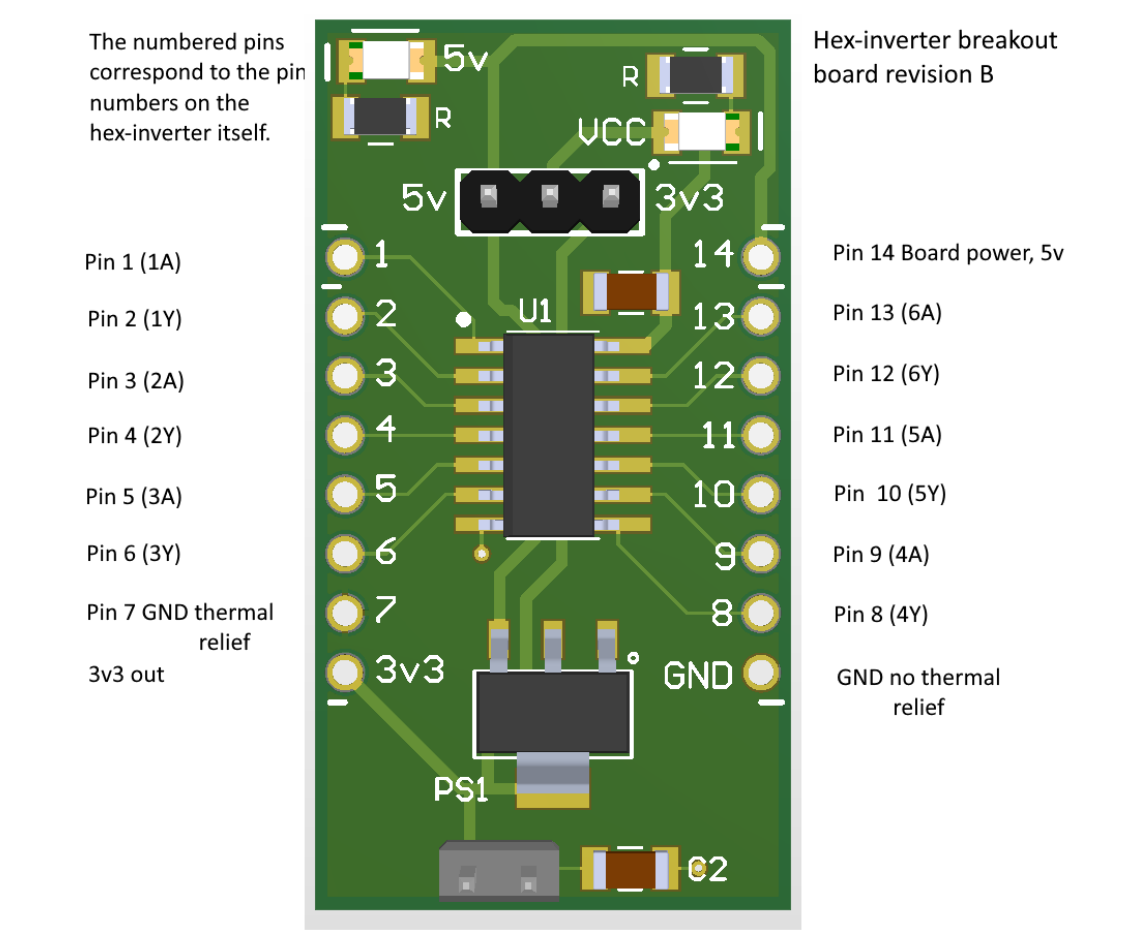
\includegraphics[scale=0.6]{figures/hex_pcb.png}
	\caption{PDN circuit block diagram from book}
	\label{idealbpfilter}
\end{figure}



\pagebreak

\section{Component listing}

We are using 555 timer board with new Hex board to 

	\begin{table}[H]
		\centering

		\begin{tabular}{c}
			\hline
			\textbf{Component Name}\\\hline
			\\
	1 x 555 timer chip\\
	1 x SN74AHC14 hex inverter \\
	Low Drop-Out (LDO) regulator (3.3 V) \\
	Hex inverter breakout board \\
	Special crosstalk test board \\
	Capacitor(Filter and Decoupling) \\
	\hline\hline
		\end{tabular}
		\caption{Labs Components}
		\label{filterspecs}
	\end{table}



\section{Calculations}


\subsection{Calculation for Hex Inverter}

\begin{figure}[H]
	\centering
	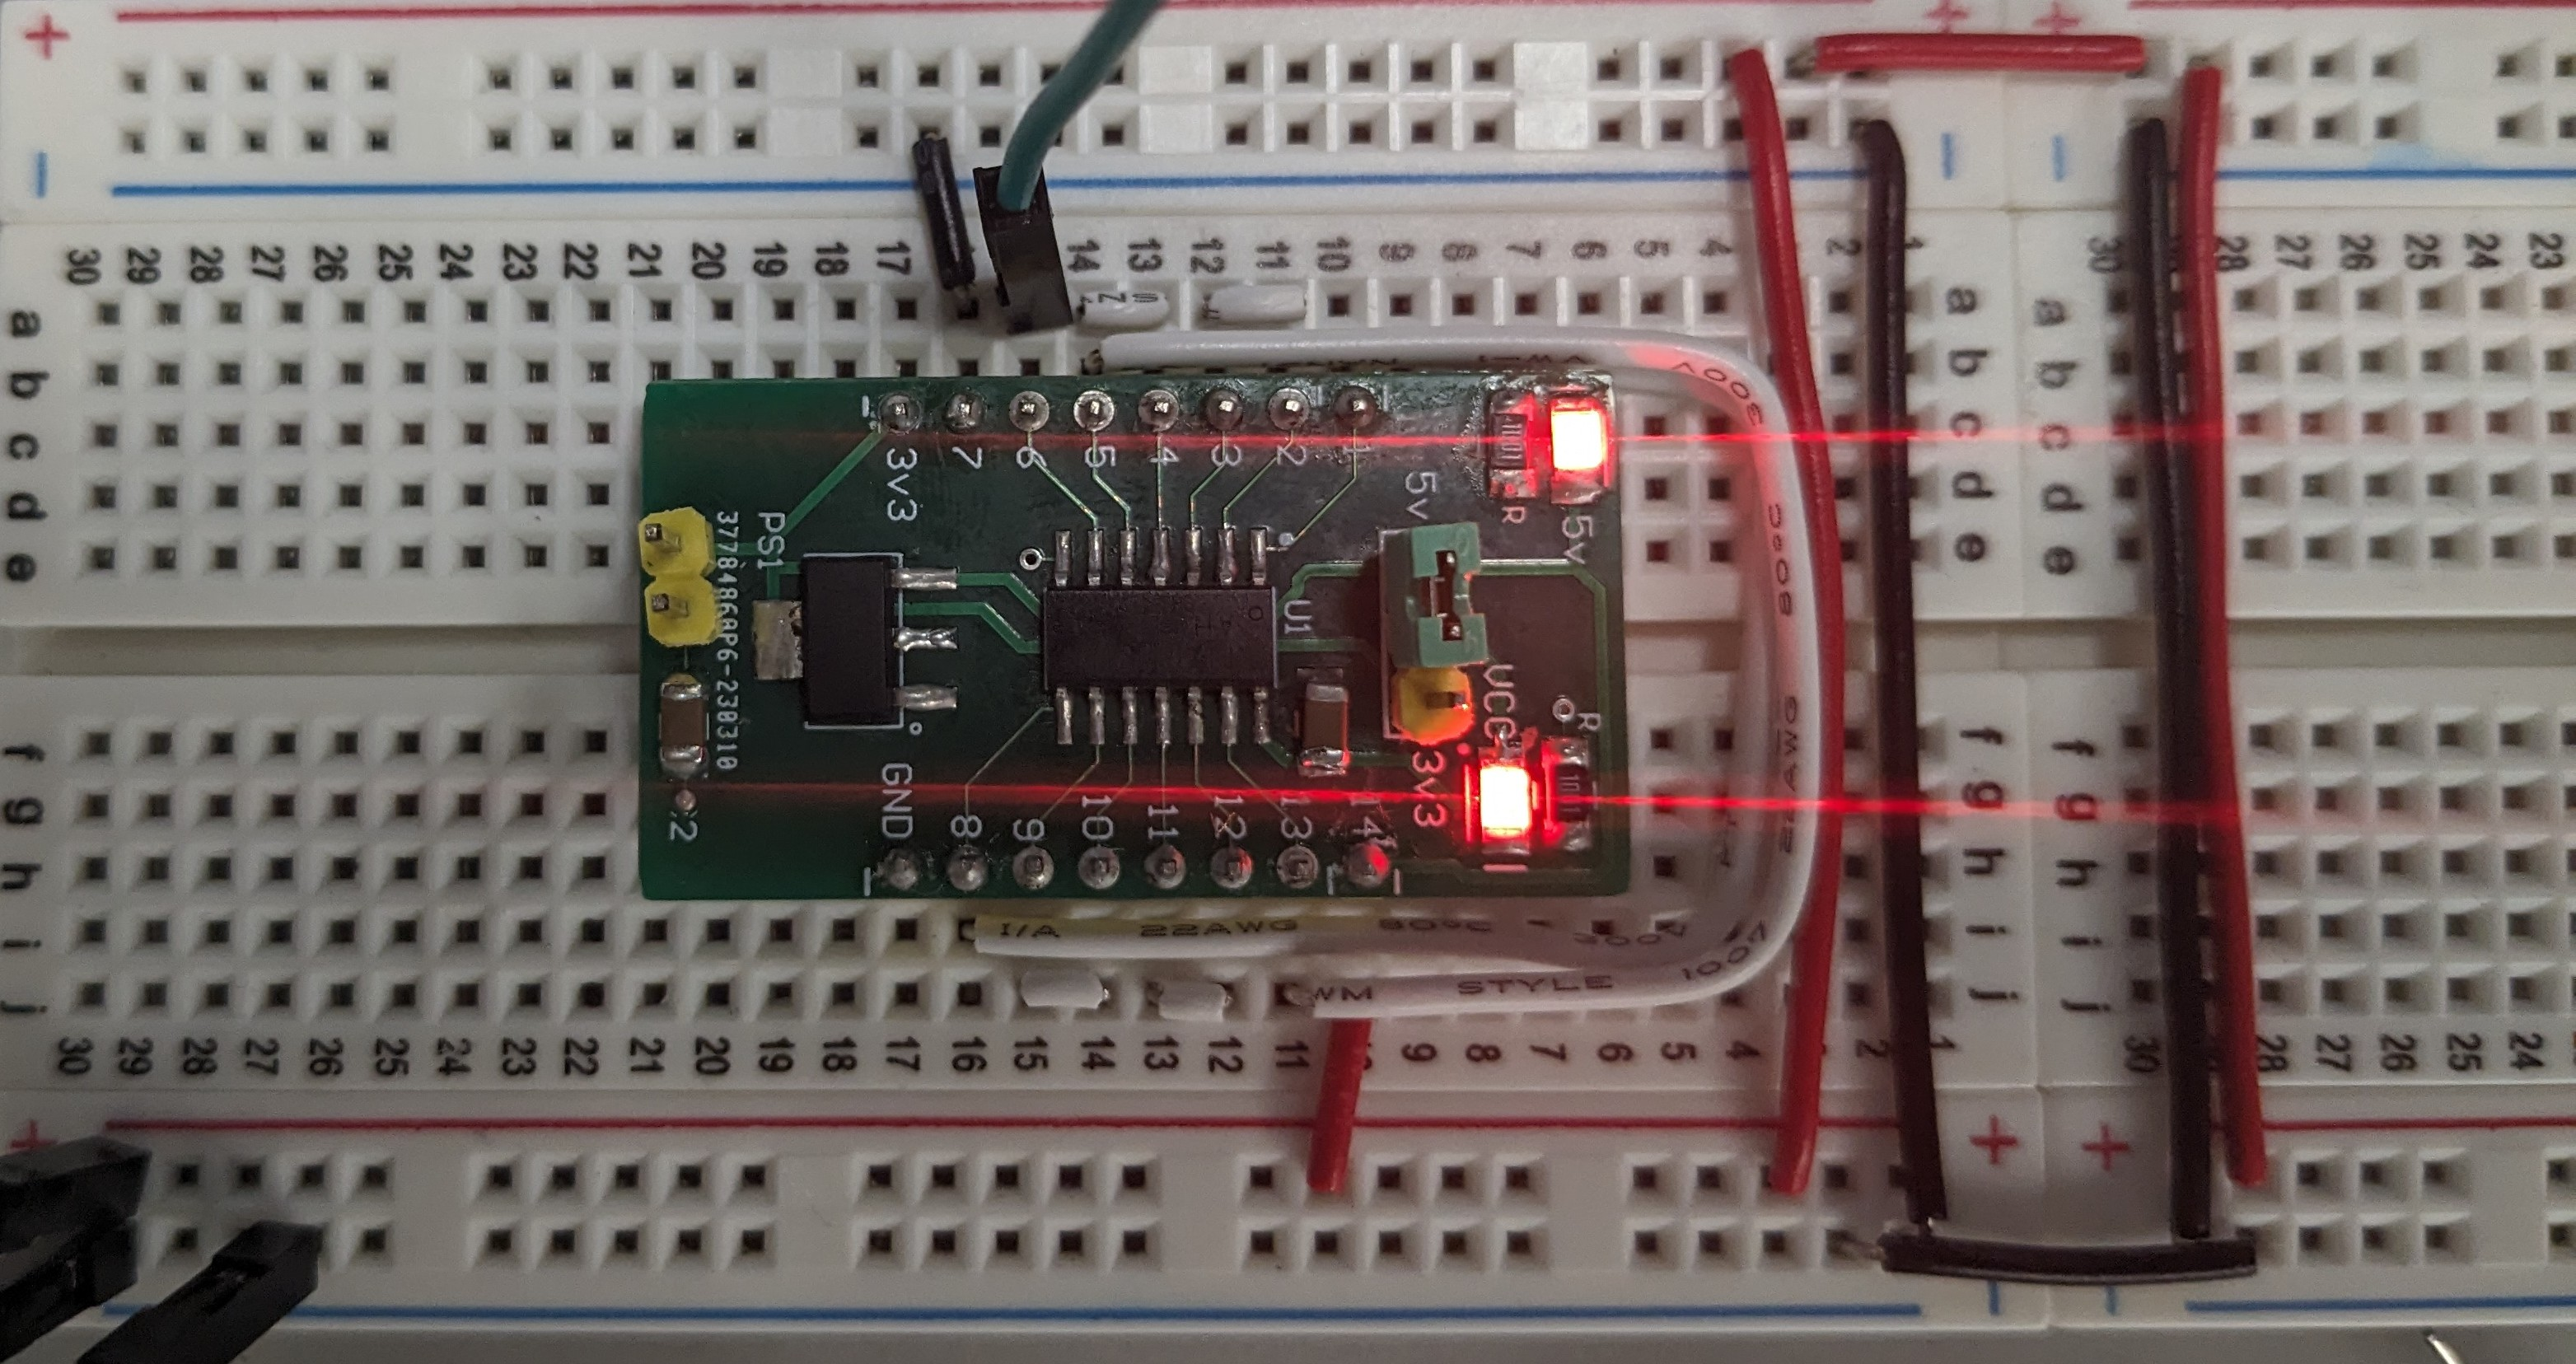
\includegraphics[scale=0.2]{figures/hexboard.jpg}
	\caption{Ring oscillator with Hex board}
	\label{hexboard}
\end{figure}

Soldered Hex Inverter (74AHC14) board of 1206 components and bringup the board and tested it by making ring occilator in following configuration 

\begin{figure}[H]
	\centering
	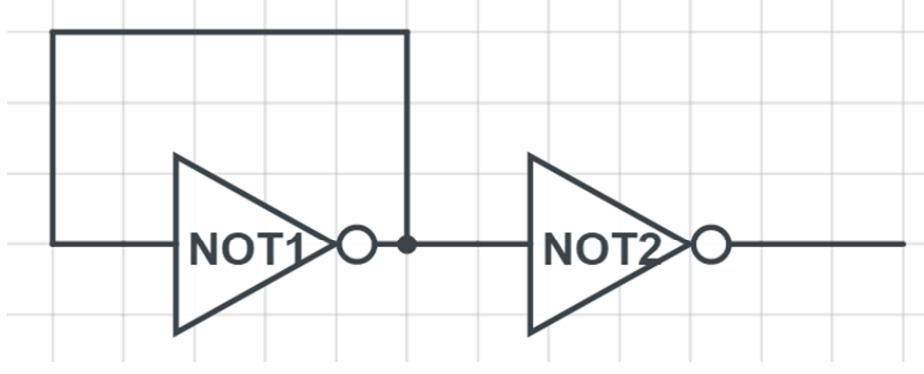
\includegraphics[scale=0.6]{figures/ring.png}
	\caption{Ring Occilator}
	\label{ring}
\end{figure}

In the PCB design, the pins labeled 'A' serve as inputs and those labeled 'Y' function as outputs. The configuration of the hex inverter includes a feedback loop from an output to an input, creating an oscillator based on the gate's propagation delay, which is specified in the datasheet to be approximately 2ns. To calculate the oscillation frequency of this hex inverter-based oscillator, one must account for both the transition from high to low and the transition from low to high, effectively doubling the propagation delay:

\begin{flalign*}
	\label{equation_th}
	&T_{total} = 2 \cdot (T_{propagation_delay})&&\\
	&T_{total} = 2 \cdot (2ns)&&\\
	&T_{total} = 4ns&&\\
	&\text{This is the total period of the Oscillations}&&\\
	&\text{Frequency of the Oscillations would be, }&&\\
	&F = \frac{1}{T_{total}}&&\\
	&F = \frac{1}{4ns}&&\\
	&F = 0.25 \cdot 10^9&&\\
	&F = 250 \cdot 10^6&&\\
	&F = 250 MHz&&\\
\end{flalign*}
Which is out of range for our oscilloscopes to measure as our scopes could measure upto 200MHz only

\begin{figure}[H]
	\centering
	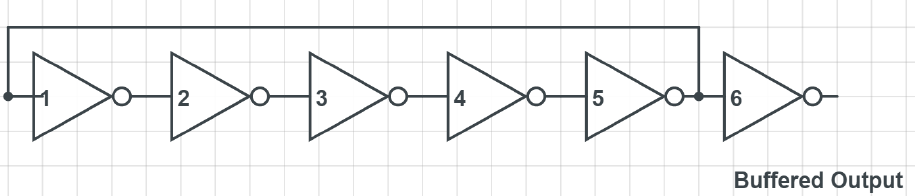
\includegraphics[scale=0.6]{figures/mul_ring.png}
	\caption{Series Ring Oscillator}
	\label{ring}
\end{figure}	

adding 6 hexinverter into series causes this propagation delay to be added in series so final propagation delay for the 6 inverter inthe serier would be around 30ns and we get the period of 30 ns plus we have to add rise and fall time for the IC also that is 5ns in our case so total time would be around 60 ns and putting that value int the formula will give us


\begin{flalign*}
	&T_{total} = 2 \cdot (T_{propagation_delay})&&\\
	&T_{total} = 2 \cdot (6 \cdot 2ns)&&\\
	&T_{total} = 24ns&&\\
	&\text{This is the total period of the Oscillations}&&\\
	&\text{Frequency of the Oscillations would be, }&&\\
	&F = \frac{1}{T_{total}}&&\\
	&F = \frac{1}{24ns}&&\\
	&F = 0.04166 \cdot 10^9&&\\
	&F = 41.66 \cdot 10^6&&\\
	&F = 41.66 MHz&&\\
\end{flalign*}

We are getting 45 MHz in practical which seem feasible as there would be some component variability and additional delays not counted\\

Here is the screenshot of the output of the ring oscillator (6 in series) 

\begin{figure}[H]
	\centering
	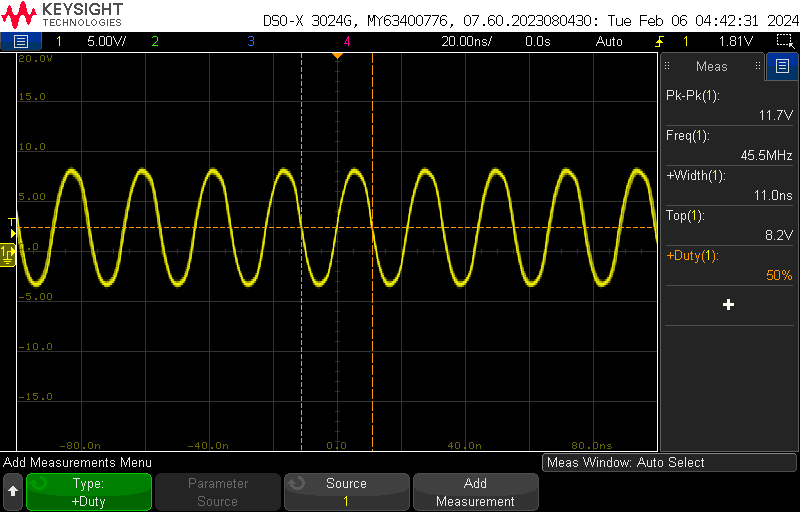
\includegraphics[scale=0.6]{figures/ring_oscillator.png}
	\caption{Ring Occilator output}
	\label{ring}
\end{figure}	

\subsection{Calculation for Hex Inverter with 555 Board}

For the next lab we need to configure the 555 timer as an astable multivibrator to output a 500 Hz signal with approximately a 50\% duty cycle, and connecting the 555 timer output to drive the hex inverter inputs. we will measure the output without any decoupling cap first\\

Triggering the oscilloscope on the hex inverter's output to measure noise levels on the quiet LOW and HIGH outputs, will give us noise of around 40mV peak to peak.

Using a 10x scope probe to capture and compare the output signal of the 555 timer and the hex inverter, shows that rise time of 555 timer is around 25nS and for hex inverter it is 5nS

\begin{figure}[H]
	\centering
	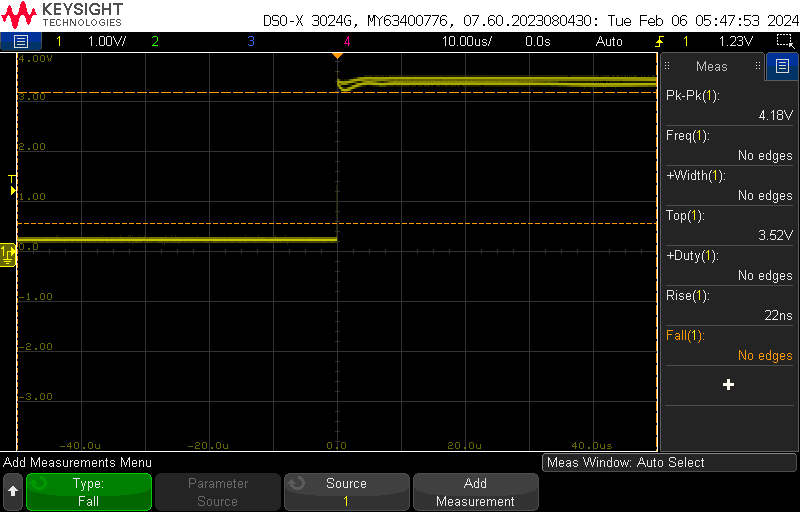
\includegraphics[scale=0.6]{figures/rise_555.png}
	\caption{555 Timer rise time}
	\label{rise555}
\end{figure}

\begin{figure}[H]
	\centering
	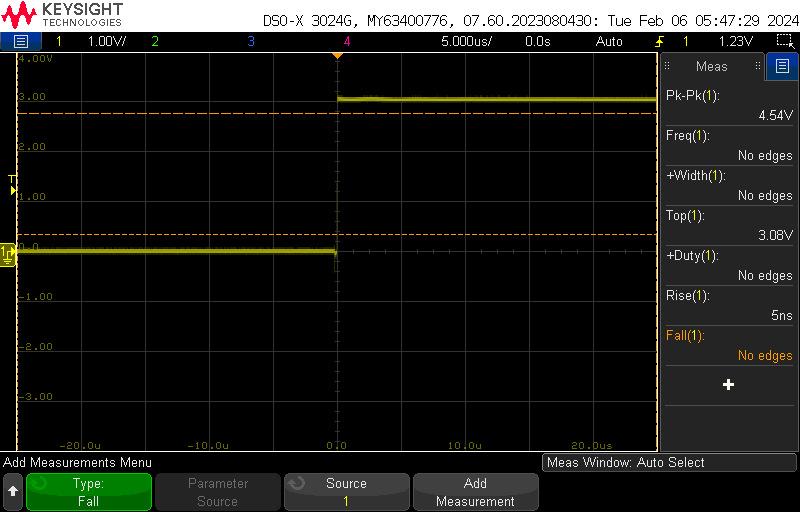
\includegraphics[scale=0.6]{figures/rise_hex.png}
	\caption{Hex inverter Rise time}
	\label{risehex}
\end{figure}


 

% Removing LEDs impacts noise on the HIGH signal.

% Experiment with adding a 1 uF capacitor near the 7414 hex inverter and observe any changes in noise levels on the quiet HIGH output.

\subsection{Calculation for Cross Talk}
\textbf{Background}
\begin{enumerate}
	\item Crosstalk is a form of interference caused by the unintended coupling between signal paths in an electronic circuit. This phenomenon can lead to the corruption of signals, resulting in operational errors and degraded performance. Crosstalk primarily occurs through two mechanisms: capacitive and inductive coupling.
	\begin{enumerate}
		\item Capacitive Crosstalk: This occurs when two conductive paths are in close proximity, allowing for the transfer of energy through a shared electric field. The coupling capacitance between the conductors can cause a signal in one conductor to induce a voltage in the adjacent conductor, particularly when there are rapid changes in the signal voltage, leading to what is known as "capacitive coupling."
		\item Inductive Crosstalk: Inductive crosstalk is the result of magnetic field interaction between conductors. When a current flows through a conductor, it generates a magnetic field around it. If there is a nearby conductor, this changing magnetic field can induce a current in the second conductor, especially if the original current changes rapidly. This effect is more pronounced at higher frequencies and with faster current changes, leading to "inductive coupling."
	\end{enumerate}
	\item Importance of Rise Time \\ 
	The rise time of a signal is a critical factor in both capacitive and inductive crosstalk. Rise time refers to the duration it takes for a signal to transition from a low to a high state (or vice versa), typically measured between the 10\% and 90\% thresholds of the signal amplitude. Faster rise times (shorter durations) mean that the signal's voltage or current changes more rapidly.

	\item Switching Noise: Fast rise times can exacerbate switching noise, which is the noise generated by the rapid changes in current or voltage within a circuit. This noise can couple into adjacent circuits, affecting their performance.
	\item 
	Crosstalk and Rise Time: As the rise time decreases (i.e., as signals switch faster), the potential for both capacitive and inductive crosstalk increases. Capacitive crosstalk is more influenced by the rate of voltage change (dv/dt), while inductive crosstalk is influenced by the rate of current change (di/dt). Thus, circuits with faster switching signals are more susceptible to crosstalk.
\end{enumerate}

\subsection{Code for Arduino}
We have to just toggle the port / perticular pins everytime we loop. as this will create switching noise into victim trace.\\

We can change the number of pins toggling by changing bits in PORTB register(For testing individual pin's impact on switching noise)
\begin{lstlisting}[language=C]
void setup() {
	// Setting all the pins to OUTPUT
	pinMode(13, OUTPUT);
	pinMode(12, OUTPUT);
	pinMode(11, OUTPUT);
	pinMode(10, OUTPUT);
	pinMode(9, OUTPUT);
	pinMode(8, OUTPUT);
}
void loop() {
	// Toggling pins every loop
	PORTB=B00111111;
	PORTB=B00000000;
}
\end{lstlisting}


\subsection{Measurement with Ground Plane:}
Lower section of board has ground plane we can attach lower part of the board with Arduino and increase individual pins one by one and measure impact of each pins causing noise on victim trace.

here are the screenshots and explanation for the output:

\begin{enumerate}
	\item Initial Observation with Pin 13:\\ Activating only pin 13, which is positioned far from the victim trace, induced a noise level of 60mV peak-to-peak on the victim trace.
	\begin{figure}[H]
		\centering
		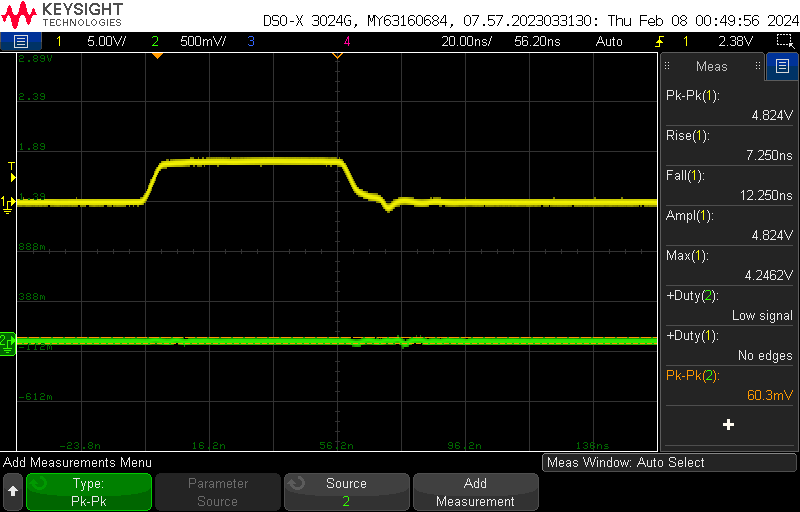
\includegraphics[scale=0.5]{figures/noise_plane_1.png}
		\caption{Noise due to 1 pins toggling(60.3mV peak to peak)}
		\label{noise_plane_1}
	\end{figure}

	\item Adding Pin 12 to the Activation:\\ Introducing pin 12 alongside pin 13 for toggling did not significantly alter the noise level on the victim trace, remaining at 60mV peak-to-peak. This outcome was expected, as both pins are located far from the victim trace.
	\begin{figure}[H]
		\centering
		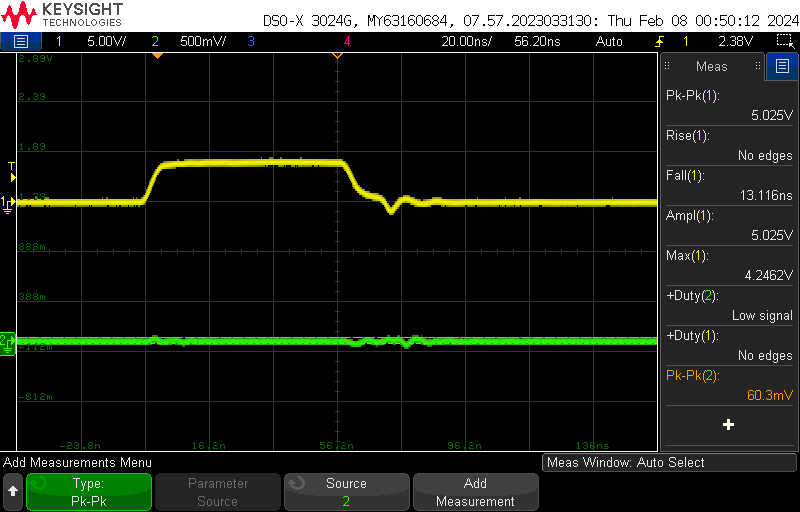
\includegraphics[scale=0.5]{figures/noise_plane_2.png}
		\caption{Noise due to 2 pins toggling(60.3mV peak to peak)}
		\label{noise_plane_2}
	\end{figure}
	
	\item Inclusion of Pin 11:\\ By toggling pins 13, 12, and now 11, an increase in noise was observed on the victim trace, with measurements showing 80.4mV peak-to-peak. This increase is attributed to pin 11's proximity to the victim trace, compared to pins 13 and 12.
	\begin{figure}[H]
		\centering
		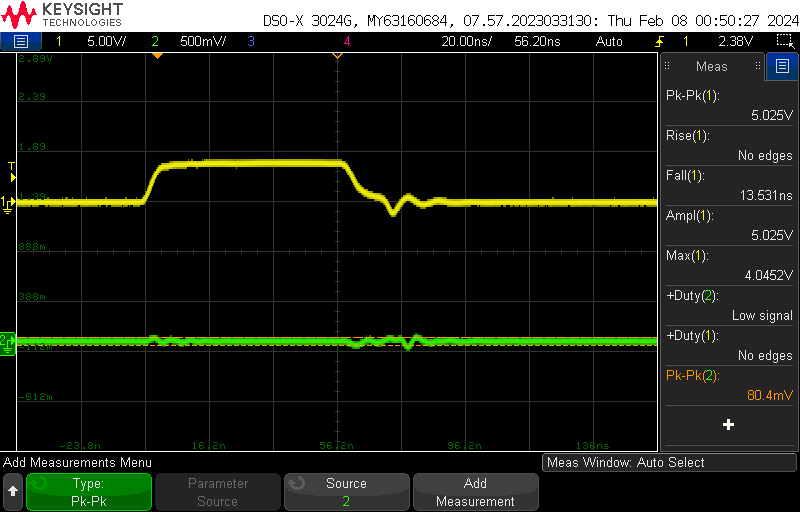
\includegraphics[scale=0.5]{figures/noise_plane_3.png}
		\caption{Noise due to 3 pins toggling(80.4mV peak to peak)}
		\label{noise_plane_3}
	\end{figure}
	
	\item Activation of Pin 10:\\ The addition of pin 10 for toggling, alongside pins 13, 12, and 11, led to a further increase in noise impact on the victim trace, reaching 120.8mV peak-to-peak. This is due to pin 10 being closer to the victim trace than pin 11.
	\begin{figure}[H]
		\centering
		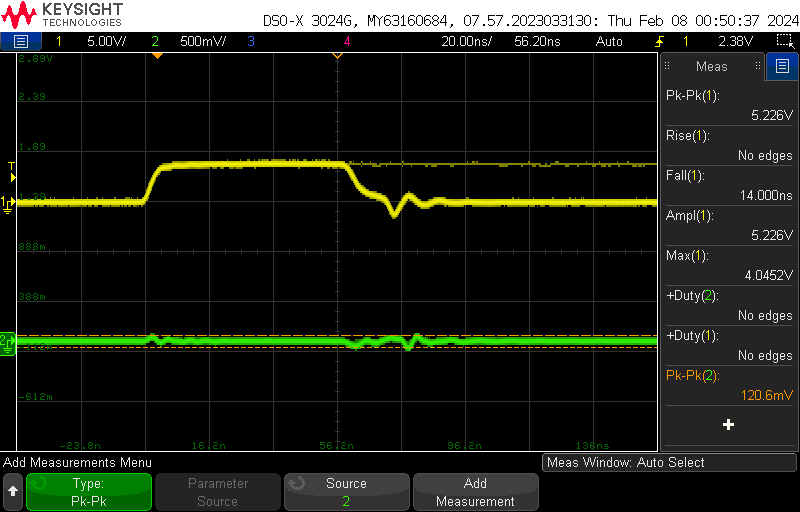
\includegraphics[scale=0.5]{figures/noise_plane_4.png}
		\caption{Noise due to 4 pins toggling(120.8mV peak to peak)}
		\label{noise_plane_4}
	\end{figure}
	
	\item Incorporating Pin 9:\\ Toggling five pins now, including pin 9 along with the previously mentioned pins, resulted in an escalated noise level on the victim trace, measuring at 140.7mV peak-to-peak. Pin 9's closer proximity to the victim trace than pin 10 explains the increased noise.
	\begin{figure}[H]
		\centering
		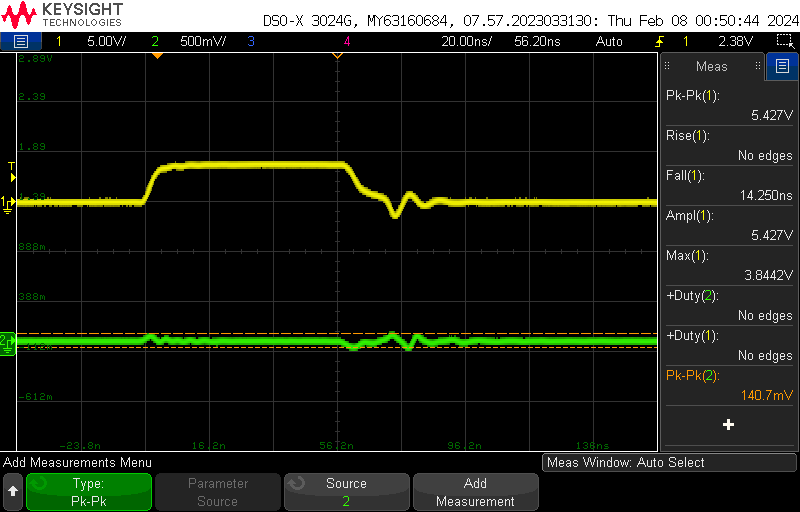
\includegraphics[scale=0.5]{figures/noise_plane_5.png}
		\caption{Noise due to 5 pins toggling(140.7mV peak to peak)}
		\label{noise_plane_5}
	\end{figure}
	
	\item Final Scenario with All Six Pins:\\ Activating all six pins for toggling, with pin 8 being the closest to the victim trace, generated the highest noise level observed in this experiment, at 341.7mV peak-to-peak. This significant increase underscores the impact of pin proximity to the victim trace on the magnitude of noise generated.
	\begin{figure}[H]
		\centering
		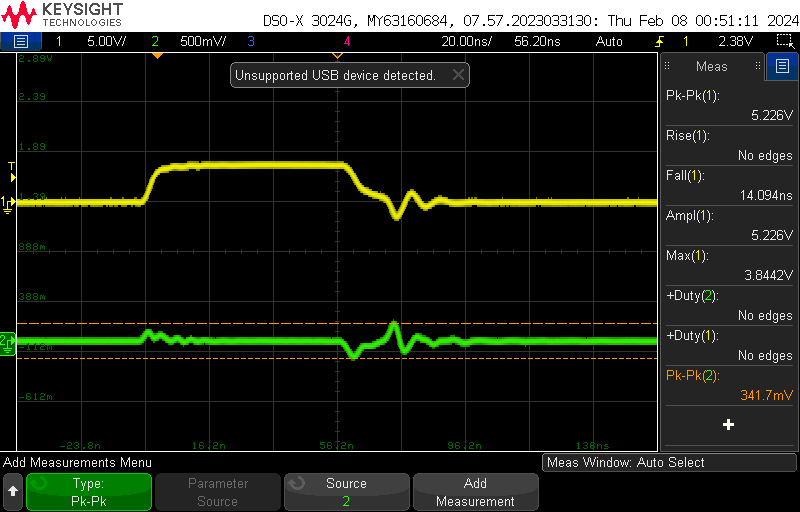
\includegraphics[scale=0.5]{figures/noise_plane_6.png}
		\caption{Noise due to all 6 pins toggling(341.7mV peak to peak)}
		\label{noise_plane_6}
	\end{figure}
	
\end{enumerate}
These observations underline the direct relationship between the proximity of toggling pins to the victim trace and the level of electromagnetic interference-induced noise



\subsection{Measurement with Continuous Return Path and no Ground Plane:}
The test board's section with a continuous return plane, the aggressor signals were driven with different simultaneous switching patterns, and the induced noise on the victim line was measured.


here are the screenshots and explanation for the output:

\begin{enumerate}
	\item The investigation extended to a section of the test board featuring a continuous return path but lacking a ground plane, focusing on the impact of various simultaneous switching patterns by aggressor signals on the induced noise within a victim line.
	\begin{figure}[H]
		\centering
		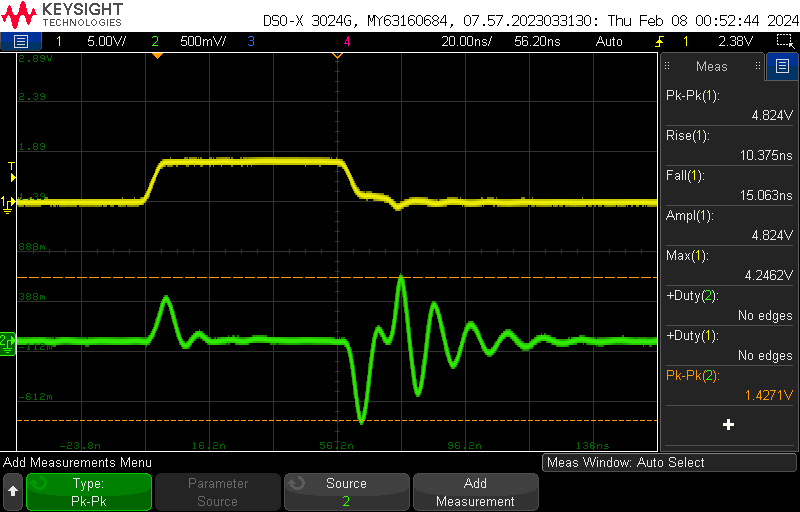
\includegraphics[scale=0.5]{figures/noise_np__cr1.png}
		\caption{Noise due to 1 pins toggling(1.427V peak to peak)}
		\label{noise_np__cr1}
	\end{figure}

	\item Incorporating Pin 12:\\ The introduction of pin 12, in conjunction with pin 13, escalated the noise to 2.33V peak-to-peak, indicating a direct correlation between the number of toggling pins and the magnitude of induced noise.
	\begin{figure}[H]
		\centering
		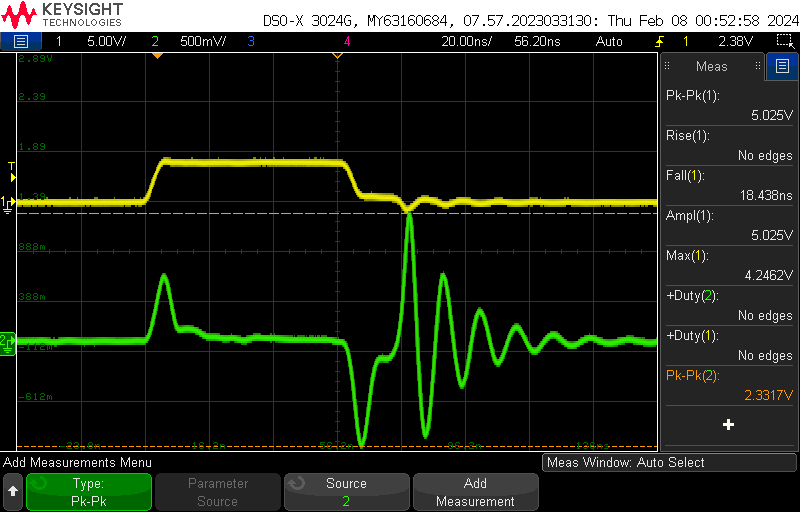
\includegraphics[scale=0.5]{figures/noise_np__cr2.png}
		\caption{Noise due to 2 pins toggling(2.33V peak to peak)}
		\label{noise_np__cr2}
	\end{figure}
	
	\item Adding Pin 11:\\ With pins 13, 12, and 11 toggling, the noise on the victim trace further increased to 3.01V peak-to-peak. This rise in noise can be attributed to pin 11's closer proximity to the victim trace compared to the previously activated pins.
	\begin{figure}[H]
		\centering
		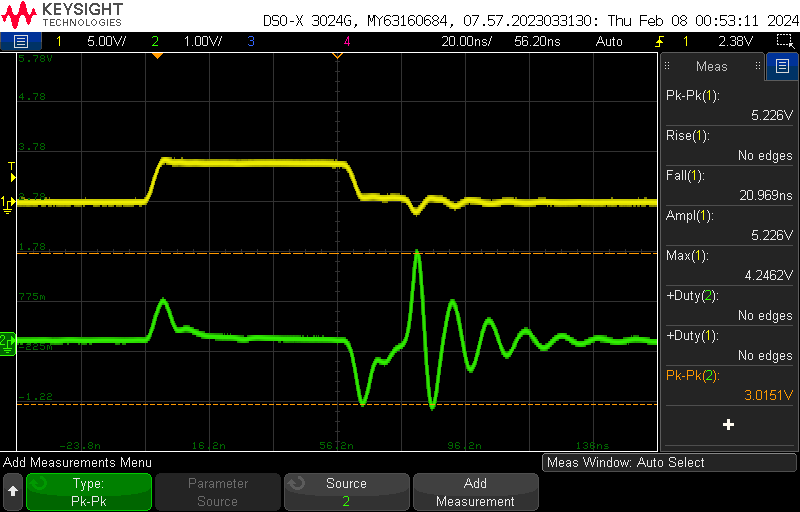
\includegraphics[scale=0.5]{figures/noise_np__cr3.png}
		\caption{Noise due to 3 pins toggling(3.01V peak to peak)}
		\label{noise_np__cr3}
	\end{figure}
	
	\item Activation of Pin 10:\\ Introducing pin 10 to the toggling sequence, alongside pins 13, 12, and 11, caused an additional noise increase on the victim trace, reaching 3.65V peak-to-peak. This was due to pin 10's closer position relative to the victim trace.
	\begin{figure}[H]
		\centering
		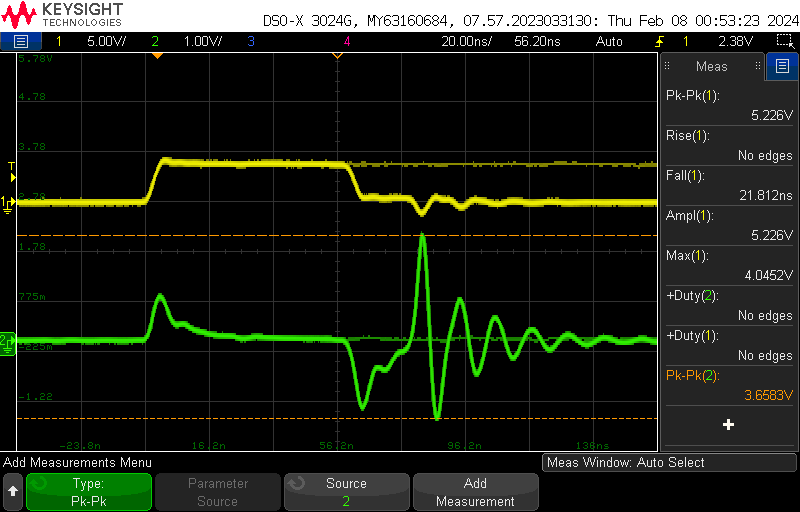
\includegraphics[scale=0.5]{figures/noise_np__cr4.png}
		\caption{Noise due to 4 pins toggling(3.65V peak to peak)}
		\label{noise_np__cr4}
	\end{figure}
	
	\item Inclusion of Pin 9:\\ Engaging five pins, including pin 9 with the others, led to a further escalated noise level of 4.22V peak-to-peak on the victim trace. The proximity of pin 9 to the victim trace was a key factor in this increased interference
	\begin{figure}[H]
		\centering
		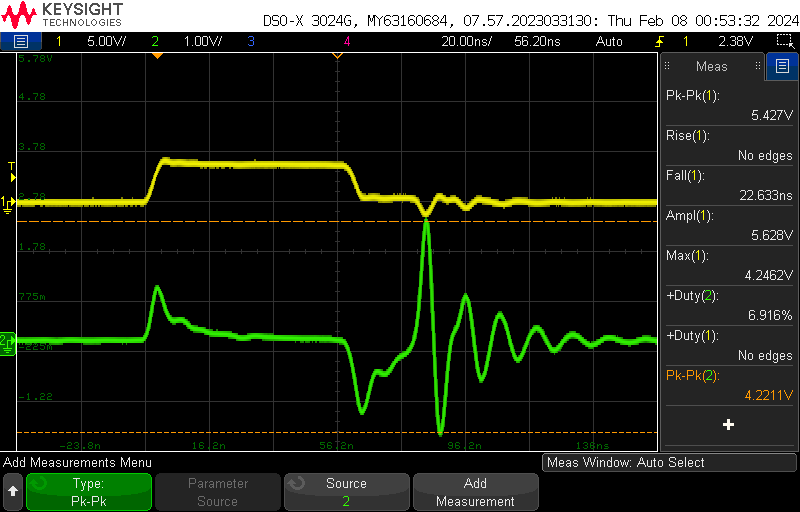
\includegraphics[scale=0.5]{figures/noise_np__cr5.png}
		\caption{Noise due to 5 pins toggling(4.22V peak to peak)}
		\label{noise_np__cr5}
	\end{figure}
	
	\item Final Setup with All Six Pins:\\ Activating all six pins for toggling, particularly with pin 8 closest to the victim trace, resulted in the highest noise level measured in this series of tests, at 4.5V peak-to-peak. This outcome emphasized the significant role of pin proximity to the victim trace in the extent of noise generation, exacerbated by the absence of a ground plane and a shared return path.
	\begin{figure}[H]
		\centering
		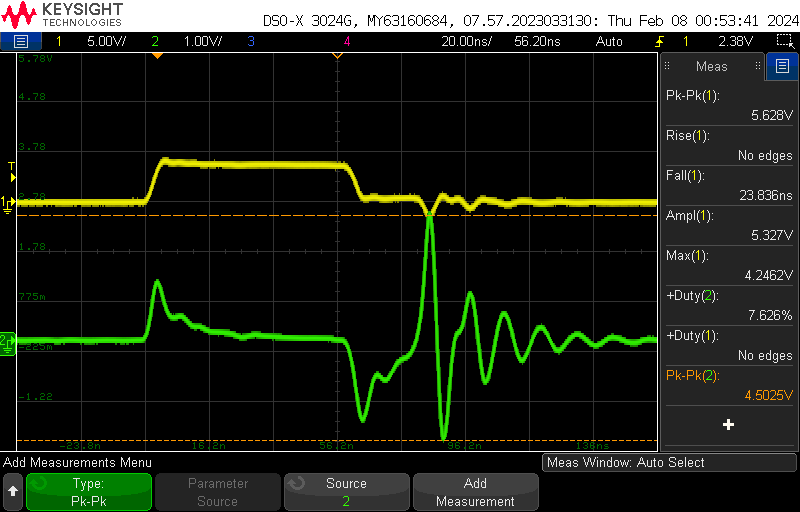
\includegraphics[scale=0.5]{figures/noise_np__cr6.png}
		\caption{Noise due to all 6 pins toggling(4.5V peak to peak)}
		\label{noise_np__cr6}
	\end{figure}
	
\end{enumerate}
Without ground plane and same return path causes 4.5V peak to peak noise ! which is not acceptable in any case.

\subsection{Measurement with Discrete Return Path and no Ground Plane:}
The middle section of the test board, featuring discrete trace paths without a continuous return plane, was used to compare the effects of shared versus separate return paths on crosstalk.


here are the screenshots and explanation for the output:

\begin{enumerate}
	\item With Pin 13 Active:\\ Engaging only pin 13, distanced from the victim trace, resulted in a noise induction of 321.6mV peak-to-peak. This was an improvement over configurations with a common return path, yet it fell short of the performance achieved with a ground plane.
	\begin{figure}[H]
		\centering
		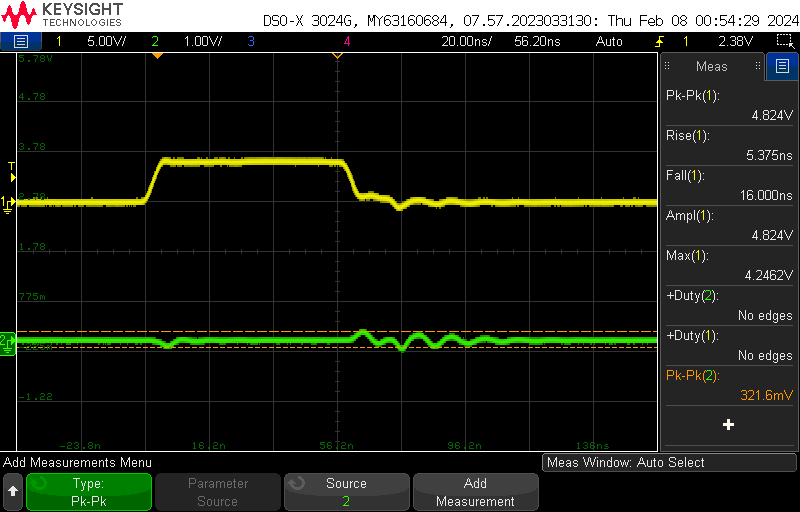
\includegraphics[scale=0.5]{figures/noise_np__sr1.png}
		\caption{Noise due to 1 pins toggling(321.6mV peak to peak)}
		\label{noise_np__sr1}
	\end{figure}

	\item Activating Pin 12:\\ Introducing pin 12 alongside pin 13 did not significantly change the noise level on the victim trace, which measured at 562.8mV peak-to-peak. This outcome aligned with expectations, given the distance of both pins from the victim trace, and it indicated an improvement compared to a common return path but was inferior to setups with a ground plane.
	\begin{figure}[H]
		\centering
		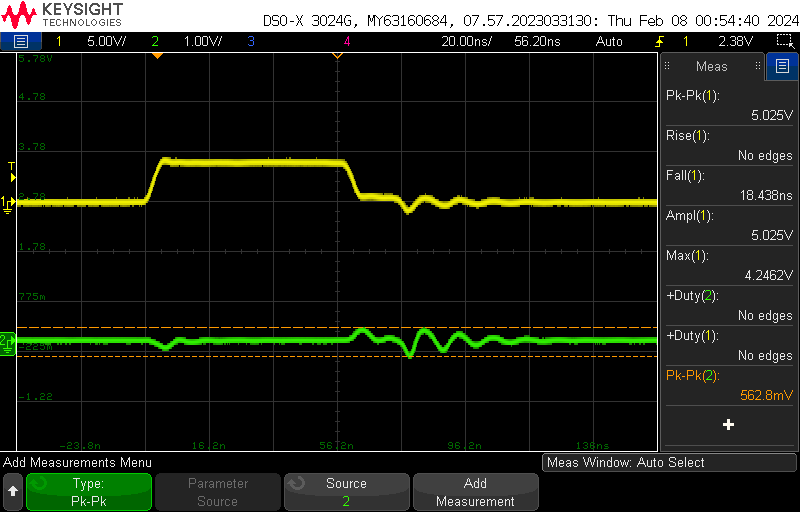
\includegraphics[scale=0.5]{figures/noise_np__sr2.png}
		\caption{Noise due to 2 pins toggling(562.8mV peak to peak)}
		\label{noise_np__sr2}
	\end{figure}
	
	\item Incorporating Pin 11:\\ The addition of pin 11 to the active set saw an uptick in noise on the victim trace to 683.4mV peak-to-peak. The proximity of pin 11 to the victim trace relative to pins 13 and 12 was the key factor in this noise increase, marking an improvement over common return path configurations but not reaching the efficacy of a ground plane.
	\begin{figure}[H]
		\centering
		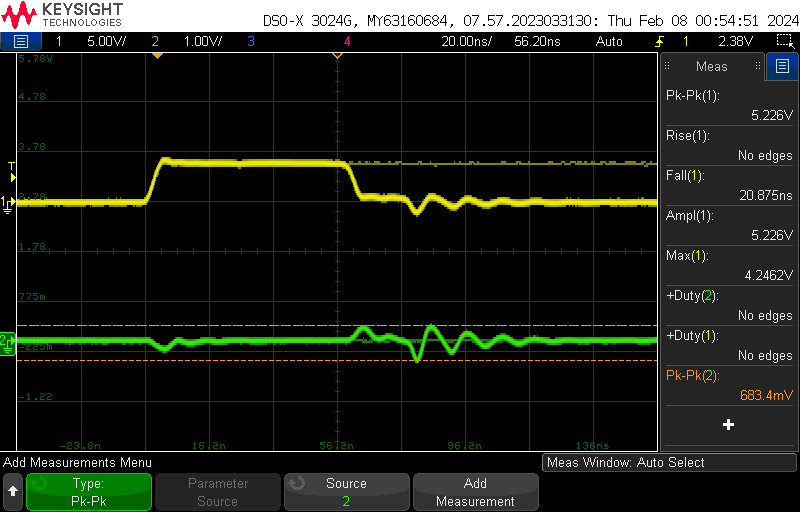
\includegraphics[scale=0.5]{figures/noise_np__sr3.png}
		\caption{Noise due to 3 pins toggling(683.4mV peak to peak)}
		\label{noise_np__sr3}
	\end{figure}
	
	\item Adding Pin 10:\\ With pin 10 now toggling alongside pins 13, 12, and 11, the noise impact on the victim trace escalated to 763.8mV peak-to-peak, attributed to pin 10's closer proximity to the victim trace. This configuration was more favorable than those with a common return path but remained less effective than those with a ground plane.
	\begin{figure}[H]
		\centering
		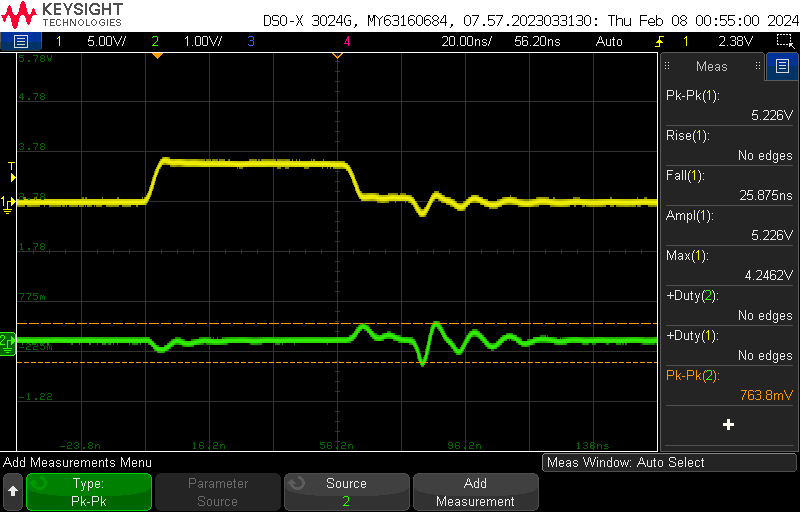
\includegraphics[scale=0.5]{figures/noise_np__sr4.png}
		\caption{Noise due to 4 pins toggling(763.8mV peak to peak)}
		\label{noise_np__sr4}
	\end{figure}
	
	\item Introducing Pin 9:\\ Activating five pins, including pin 9, heightened the noise level on the victim trace to 924.6mV peak-to-peak. Pin 9's nearness to the victim trace explained the increased interference, showcasing an improvement over scenarios with a common return path but still underperforming compared to ground plane arrangements.
	\begin{figure}[H]
		\centering
		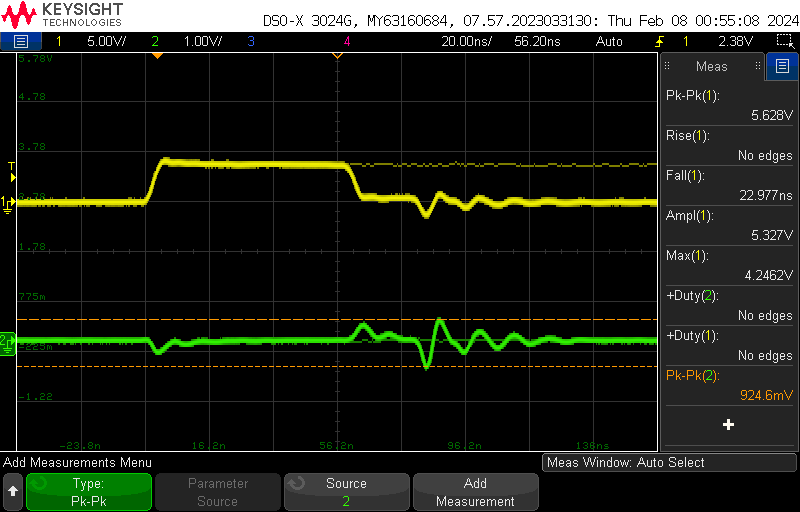
\includegraphics[scale=0.5]{figures/noise_np__sr5.png}
		\caption{Noise due to 5 pins toggling(924.6mV peak to peak)}
		\label{noise_np__sr5}
	\end{figure}
	
	\item Final Configuration with Six Pins:\\ Engaging all six pins for toggling, especially with pin 8 nearest to the victim trace, produced the highest noise level in the experiment, at 1.047V peak-to-peak. This underscored the significant role of pin proximity in noise generation, yielding better results than common return path setups but not matching the effectiveness of a ground plane presence.
	\begin{figure}[H]
		\centering
		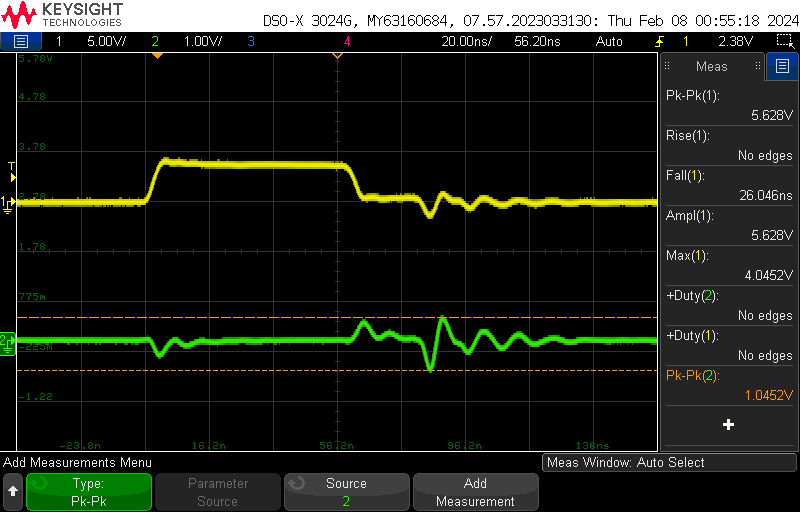
\includegraphics[scale=0.5]{figures/noise_np__sr6.png}
		\caption{Noise due to all 6 pins toggling(1.047V peak to peak)}
		\label{noise_np__sr6}
	\end{figure}
	
\end{enumerate}
This shows that we should ideally use ground plane, and if not, priorities separate signal return path.

\section{Conclusion}

The lab was about studying noise in electronic circuits, focusing on how noise is created, moves, and can be reduced. The main parts of the study included working with hex inverter circuits, using a 555 timer IC to make signals at specific frequencies, and looking at how crosstalk affects PCB designs. The goal was to see how different ways of building circuits can change how they work and how much noise they make.\\

Main Findings:\\
\begin{enumerate}
	\item Signal Transition Times:\\ The lab showed that how quickly signals change (rise and fall times) can make more noise. This means when designing circuits, it's important to think about how these changes can cause noise.
	\item Decoupling Capacitors:\\ The use of decoupling capacitors was important for reducing noise. Putting these capacitors in the right spots is key to reducing noise and keeping the circuit stable.
	\item Crosstalk:\\ The experiments helped understand crosstalk, which happens when signals in nearby wires interfere with each other. The results showed that the way wires are laid out on a PCB can make a big difference in reducing this kind of interference.
	\item Circuit Design:\\ Building and studying the hex inverter and 555 timer circuits showed that the choice of components and how the circuit is put together can affect noise and how well the circuit works. This part of the lab emphasized making good design choices to reduce noise and improve reliability.
\end{enumerate}

\textbf{Conclusion:}\\

The lab made it clear how important it is to understand noise in electronic circuits and how to reduce it. It showed the need to carefully choose and place components, and how the layout of a PCB can prevent crosstalk. These lessons are crucial for making circuits that work well and have less noise.


Crosstalk board:

\begin{figure}[H]
	\centering
	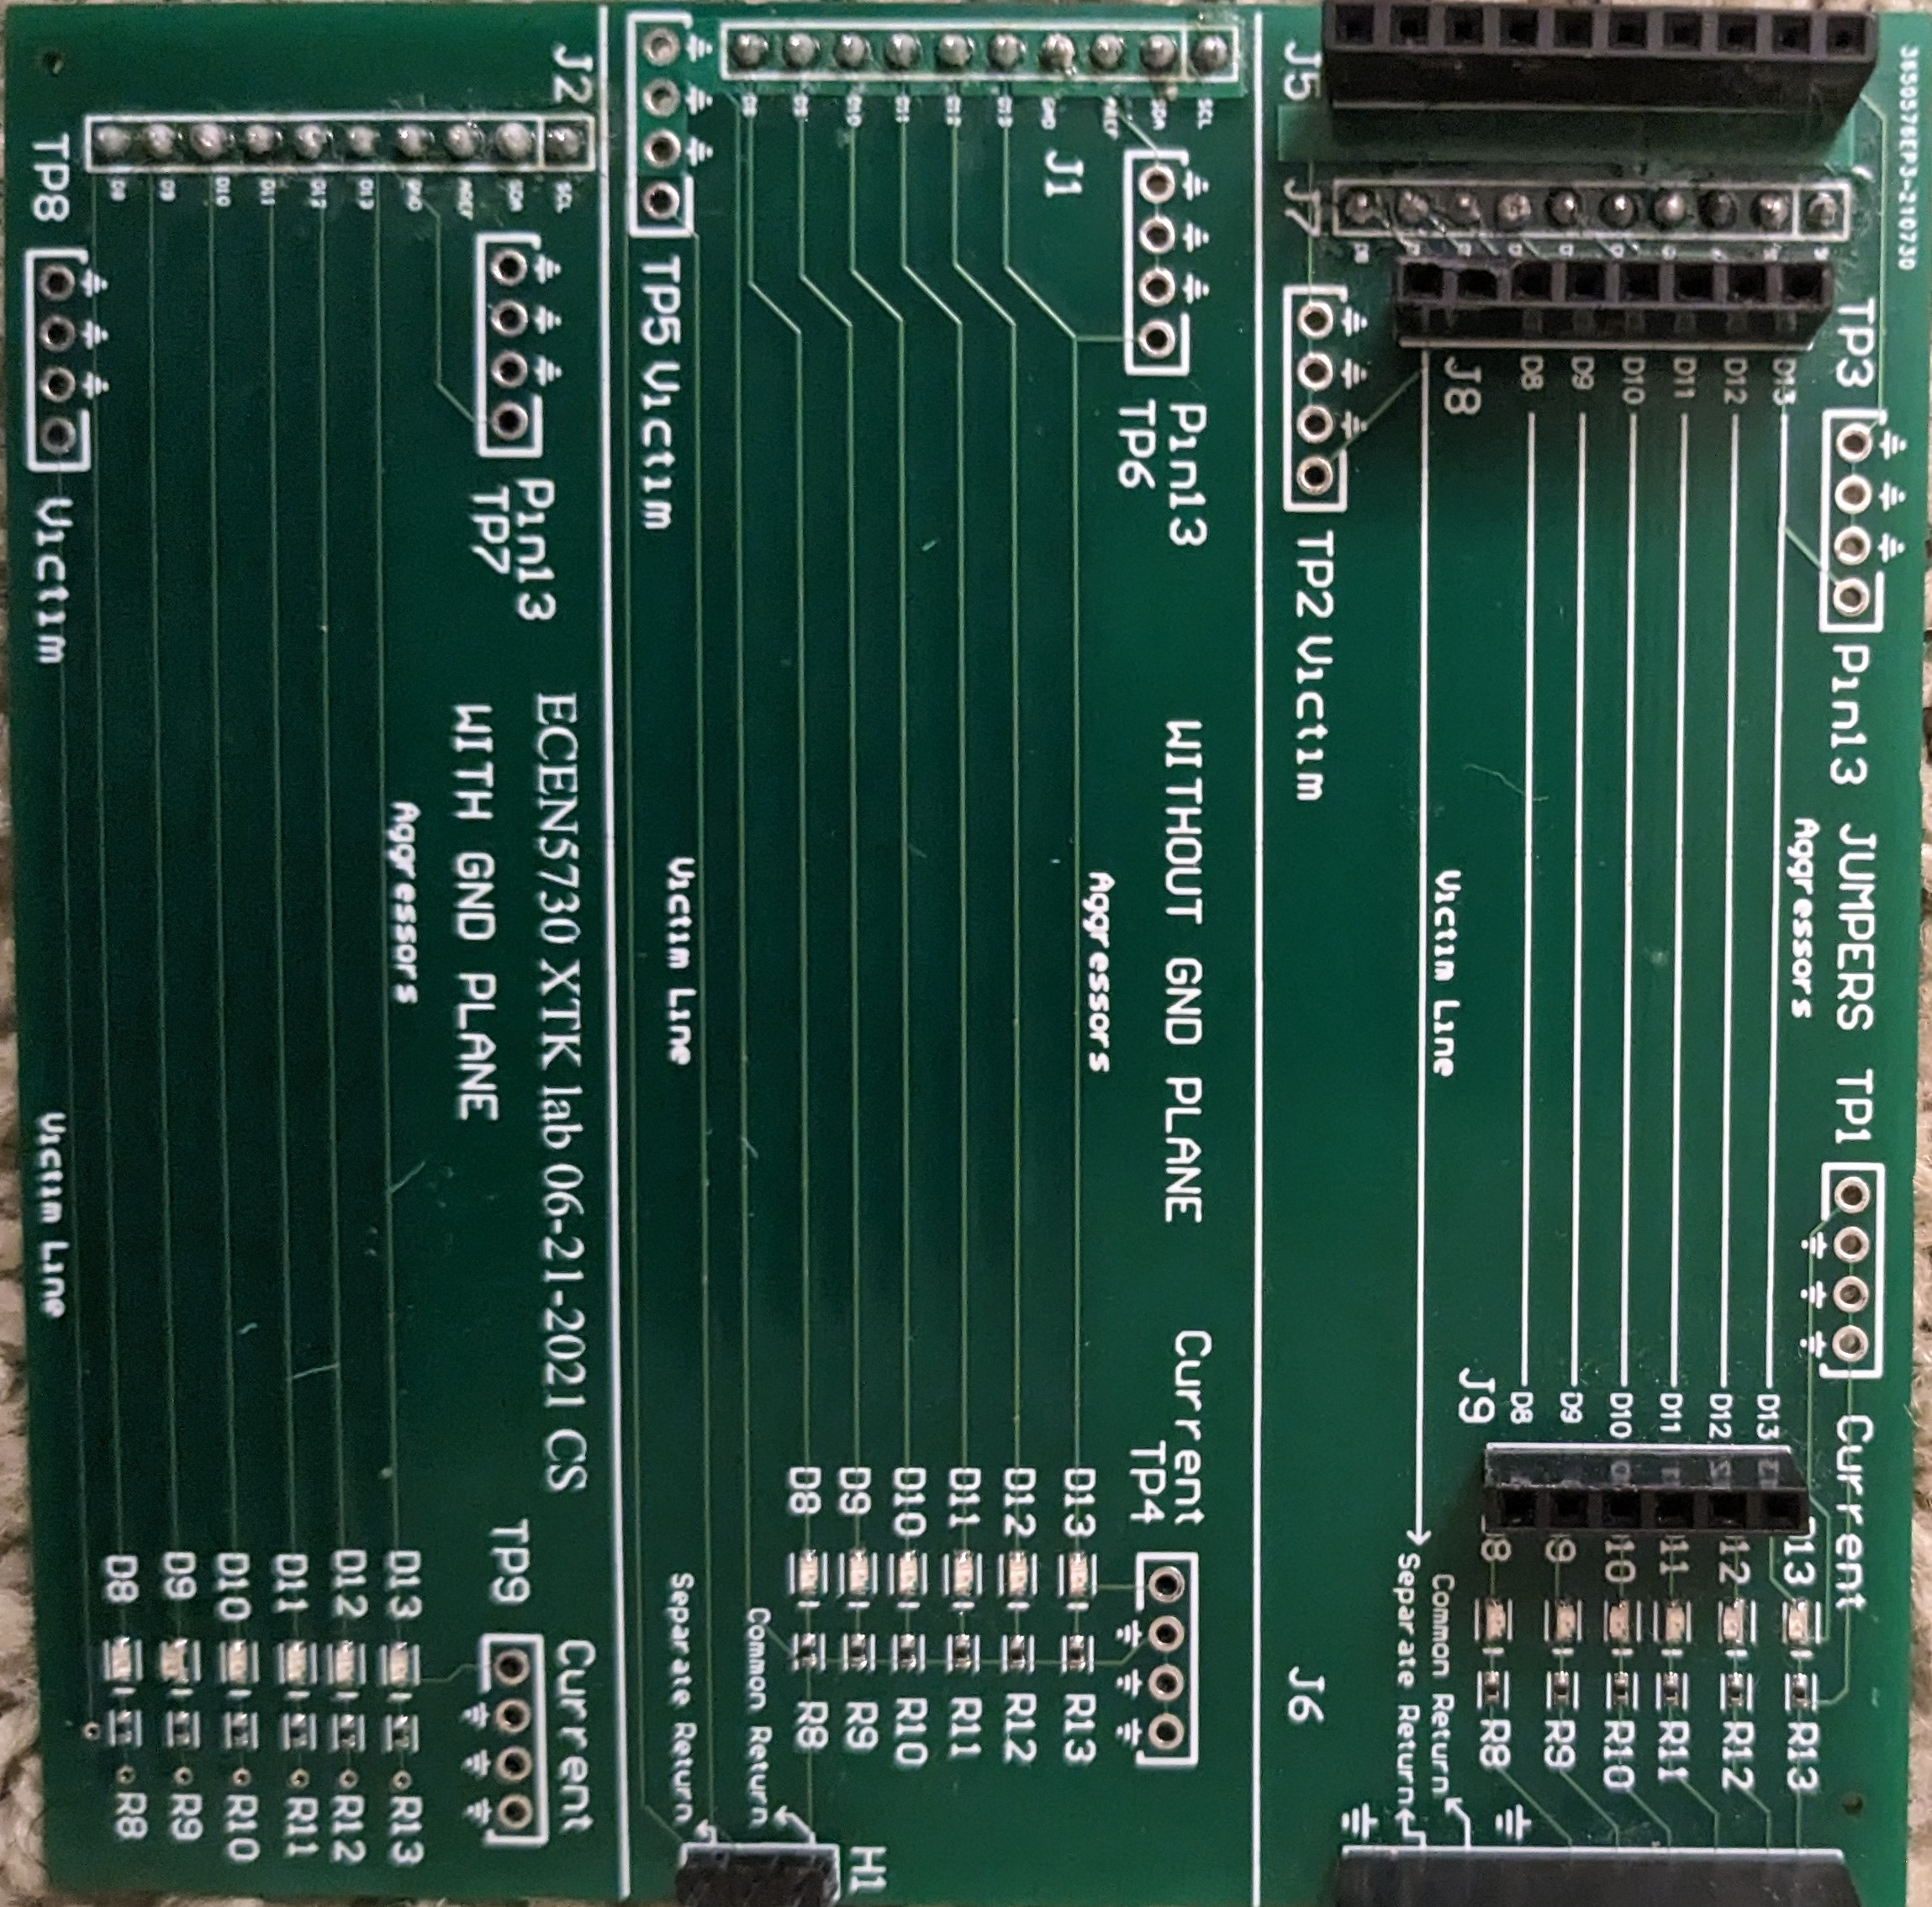
\includegraphics[scale=0.2]{figures/crosstalk.jpg}
	\caption{Crosstalk board}
	\label{crosstalk}
\end{figure}

\hrule






%---------------------------------------------------------------------------
\end{document}
-
